%brent's poster layout :)

\documentclass[article,30pt,extrafontsizes]{memoir}

%utf-8 seems to be important
\usepackage[utf8]{inputenc}
\usepackage[T1]{fontenc}
\usepackage{palatino}
\usepackage{multicol}
\usepackage{graphicx}
\usepackage{blindtext,xcolor}
\usepackage{framed}
\usepackage{color}

%For figure and table placement
\usepackage{float}
\floatplacement{figure}{H}
\floatplacement{table}{H}

%spacing between figure/ table and caption
\setlength{\abovecaptionskip}{0.4in}
\setlength{\belowcaptionskip}{0.1in}
\captionnamefont{\footnotesize\sffamily\bfseries}
\captiontitlefont{\footnotesize\sffamily}

%define column options
\setlength{\columnseprule}{1pt}
\def\columnseprulecolor{\color{red}}
\setsubsubsecheadstyle{\small\color{red}\textbf}% Set \section style
\setsecheadstyle{\small\color{red}}
\setsecnumformat{}
\def\sectionmark#1{\markboth{#1}{#1}}

%-----------------------------------------------------

%define poster size
\usepackage[paperwidth=45in,paperheight=38in, text={7in,10in},centering]{geometry}

\geometry{
left=5mm,
right=5mm,
top=0mm,
bottom=5mm,
headheight=0mm,
}

\thispagestyle{empty}

\usepackage[style=numeric,backend=biber]{biblatex}
\renewcommand*{\bibfont}{\tiny}

\bibliography{MyLibrary}

\counterwithout{section}{chapter}
\makechapterstyle{mydefault}{
\addtocounter{secnumdepth}{2}
\setsecheadstyle{\Large\color{red}\textbf}
\setsubsecheadstyle{\itshape}
\setsubsubsecheadstyle{\itshape}
}

\setlength\parindent{10mm}
\setlength\hangindent{10mm}

\chapterstyle{mydefault}

\defbibheading{bibliography}[\bibname]{%
\section*{#1}%
\markboth{#1}{#1}}


\AtBeginDocument{%
  \renewcommand{\bibname}{References}
}


%define column spacing
\setlength\columnsep{1.2in}

%spacing after section head title
\setaftersecskip{0.3in}
\setbeforesecskip{0.5in}
\setlength\textfloatsep{0.1in}
\setlength\floatsep{0.1in}
\setlength\intextsep{0.1in}
\setlength{\parskip}{0pt}

%for shading the top
\definecolor{shadecolor}{gray}{0.9}


%begin the document
\begin{document}


% group which adds title author and other infor
% Used instead of \maketitle for better spacing options
\begin{shaded}
\begingroup
  \centering
  \huge\textbf{Identifying relationships among catchment land cover characteristics,
active layer properties and lake hydroecology in Old Crow Flats, Yukon,
Canada}\\[0.3in]
  \Large W. Brent Thorne\footnote{1}; Kevin W. Turner\footnote{2}\par
\endgroup
\vspace{1.2in}
% end title section -------------------
  \end{shaded}

% Brgin body of poster
\begin{multicols*}{3}
\small{\noindent
\section{Introduction}\label{introduction}

Lorem ipsum dolor sit amet, \autocite{holden_identifying_2012}
consectetur adipiscing elit, sed do eiusmod tempor incididunt ut labore
et dolore magna aliqua. Phasellus vestibulum lorem sed risus ultricies
tristique nulla. Mauris vitae ultricies leo integer malesuada nunc vel
risus commodo. Suspendisse potenti nullam ac tortor vitae. Enim nunc
faucibus a pellentesque sit amet porttitor eget.

\section{Study Site}\label{study-site}

Here is a map made to show the study site using \texttt{ggplot2},
\texttt{ggspatial}, and \texttt{rgdal}. Lorem ipsum dolor sit amet,
\autocite{middleton_geological_nodate} consectetur adipiscing elit, sed
do eiusmod tempor incididunt ut labore et dolore magna aliqua. Phasellus
vestibulum lorem sed risus ultricies tristique nulla. Mauris vitae
ultricies leo integer malesuada nunc vel risus commodo. Suspendisse
potenti nullam ac tortor vitae. Enim nunc faucibus a pellentesque sit
amet porttitor eget.

\begin{figure}

{\centering 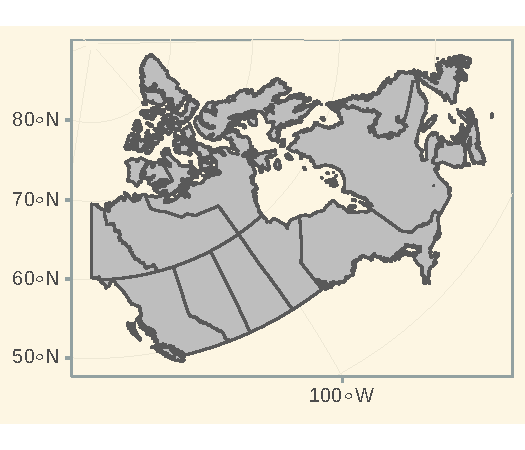
\includegraphics[width=0.8\linewidth]{skeleton_files/figure-latex/unnamed-chunk-2-1} 

}

\caption{This is a map of Canada, projected using the NAD 83 UTM Zone 7 Datum.}\label{fig:unnamed-chunk-2}
\end{figure}

\section{Objectives}\label{objectives}

\begin{enumerate}
\def\labelenumi{\arabic{enumi}.}
\tightlist
\item
  Here is my first obective.
\item
  Here is my second objective.
\item
  Finally, my third objectives.
\end{enumerate}

\section{Methods}\label{methods}

Lacinia quis vel eros donec ac odio tempor. Vel quam elementum pulvinar
etiam non quam lacus suspendisse. Nec tincidunt praesent semper feugiat
nibh sed pulvinar. Neque ornare aenean euismod elementum. Vel fringilla
est ullamcorper eget nulla. Sollicitudin aliquam ultrices sagittis orci
a. Maecenas accumsan lacus vel facilisis volutpat est velit. Sed sed
risus pretium quam vulputate dignissim. Convallis posuere morbi leo urna
molestie. Cursus vitae congue mauris rhoncus. Vitae ultricies leo
integer malesuada nunc. Est lorem ipsum dolor sit amet consectetur
adipiscing. Enim sit amet venenatis urna cursus eget nunc.

Elementum facilisis leo vel fringilla est ullamcorper eget nulla. Vitae
congue eu consequat ac felis donec et. Morbi tincidunt ornare massa
eget. Iaculis nunc sed augue lacus viverra vitae congue eu. Donec massa
sapien faucibus et molestie. Neque egestas congue quisque egestas diam.
Lectus quam id leo in vitae turpis massa. Sodales ut etiam sit amet.
Posuere lorem ipsum dolor sit amet consectetur. Ullamcorper dignissim
cras tincidunt lobortis feugiat vivamus. Amet commodo nulla facilisi
nullam vehicula ipsum. Magna ac placerat vestibulum lectus mauris
ultrices eros. Sodales ut eu sem integer vitae justo eget magna.
Malesuada bibendum arcu vitae elementum.

\section{Results}\label{results}

Sagittis purus sit amet volutpat consequat mauris. Lobortis mattis
aliquam faucibus purus. Libero enim sed faucibus turpis in eu. Massa
placerat duis ultricies lacus sed turpis tincidunt id. Arcu dictum
varius duis at consectetur lorem done.

\begin{figure}

{\centering 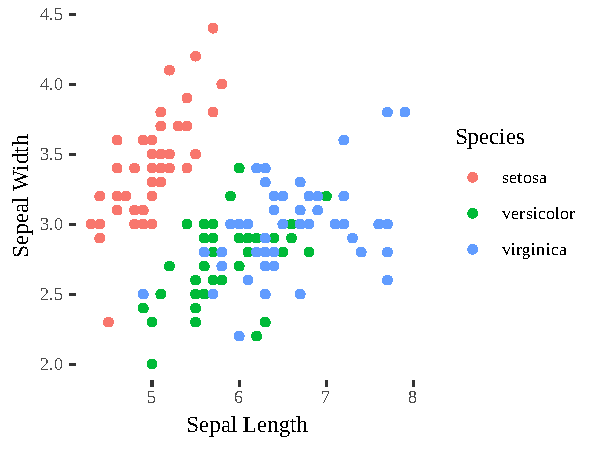
\includegraphics[width=0.6\linewidth]{skeleton_files/figure-latex/unnamed-chunk-3-1} 

}

\caption{This is a typical ggplot2 example using the iris dataset provided in R.}\label{fig:unnamed-chunk-3}
\end{figure}

Sagittis purus sit amet volutpat consequat mauris. Lobortis mattis
aliquam faucibus purus. Libero enim sed faucibus turpis in eu. Massa
placerat duis ultricies lacus sed turpis tincidunt id. Arcu dictum
varius duis at consectetur lorem done.

\begin{figure}

{\centering 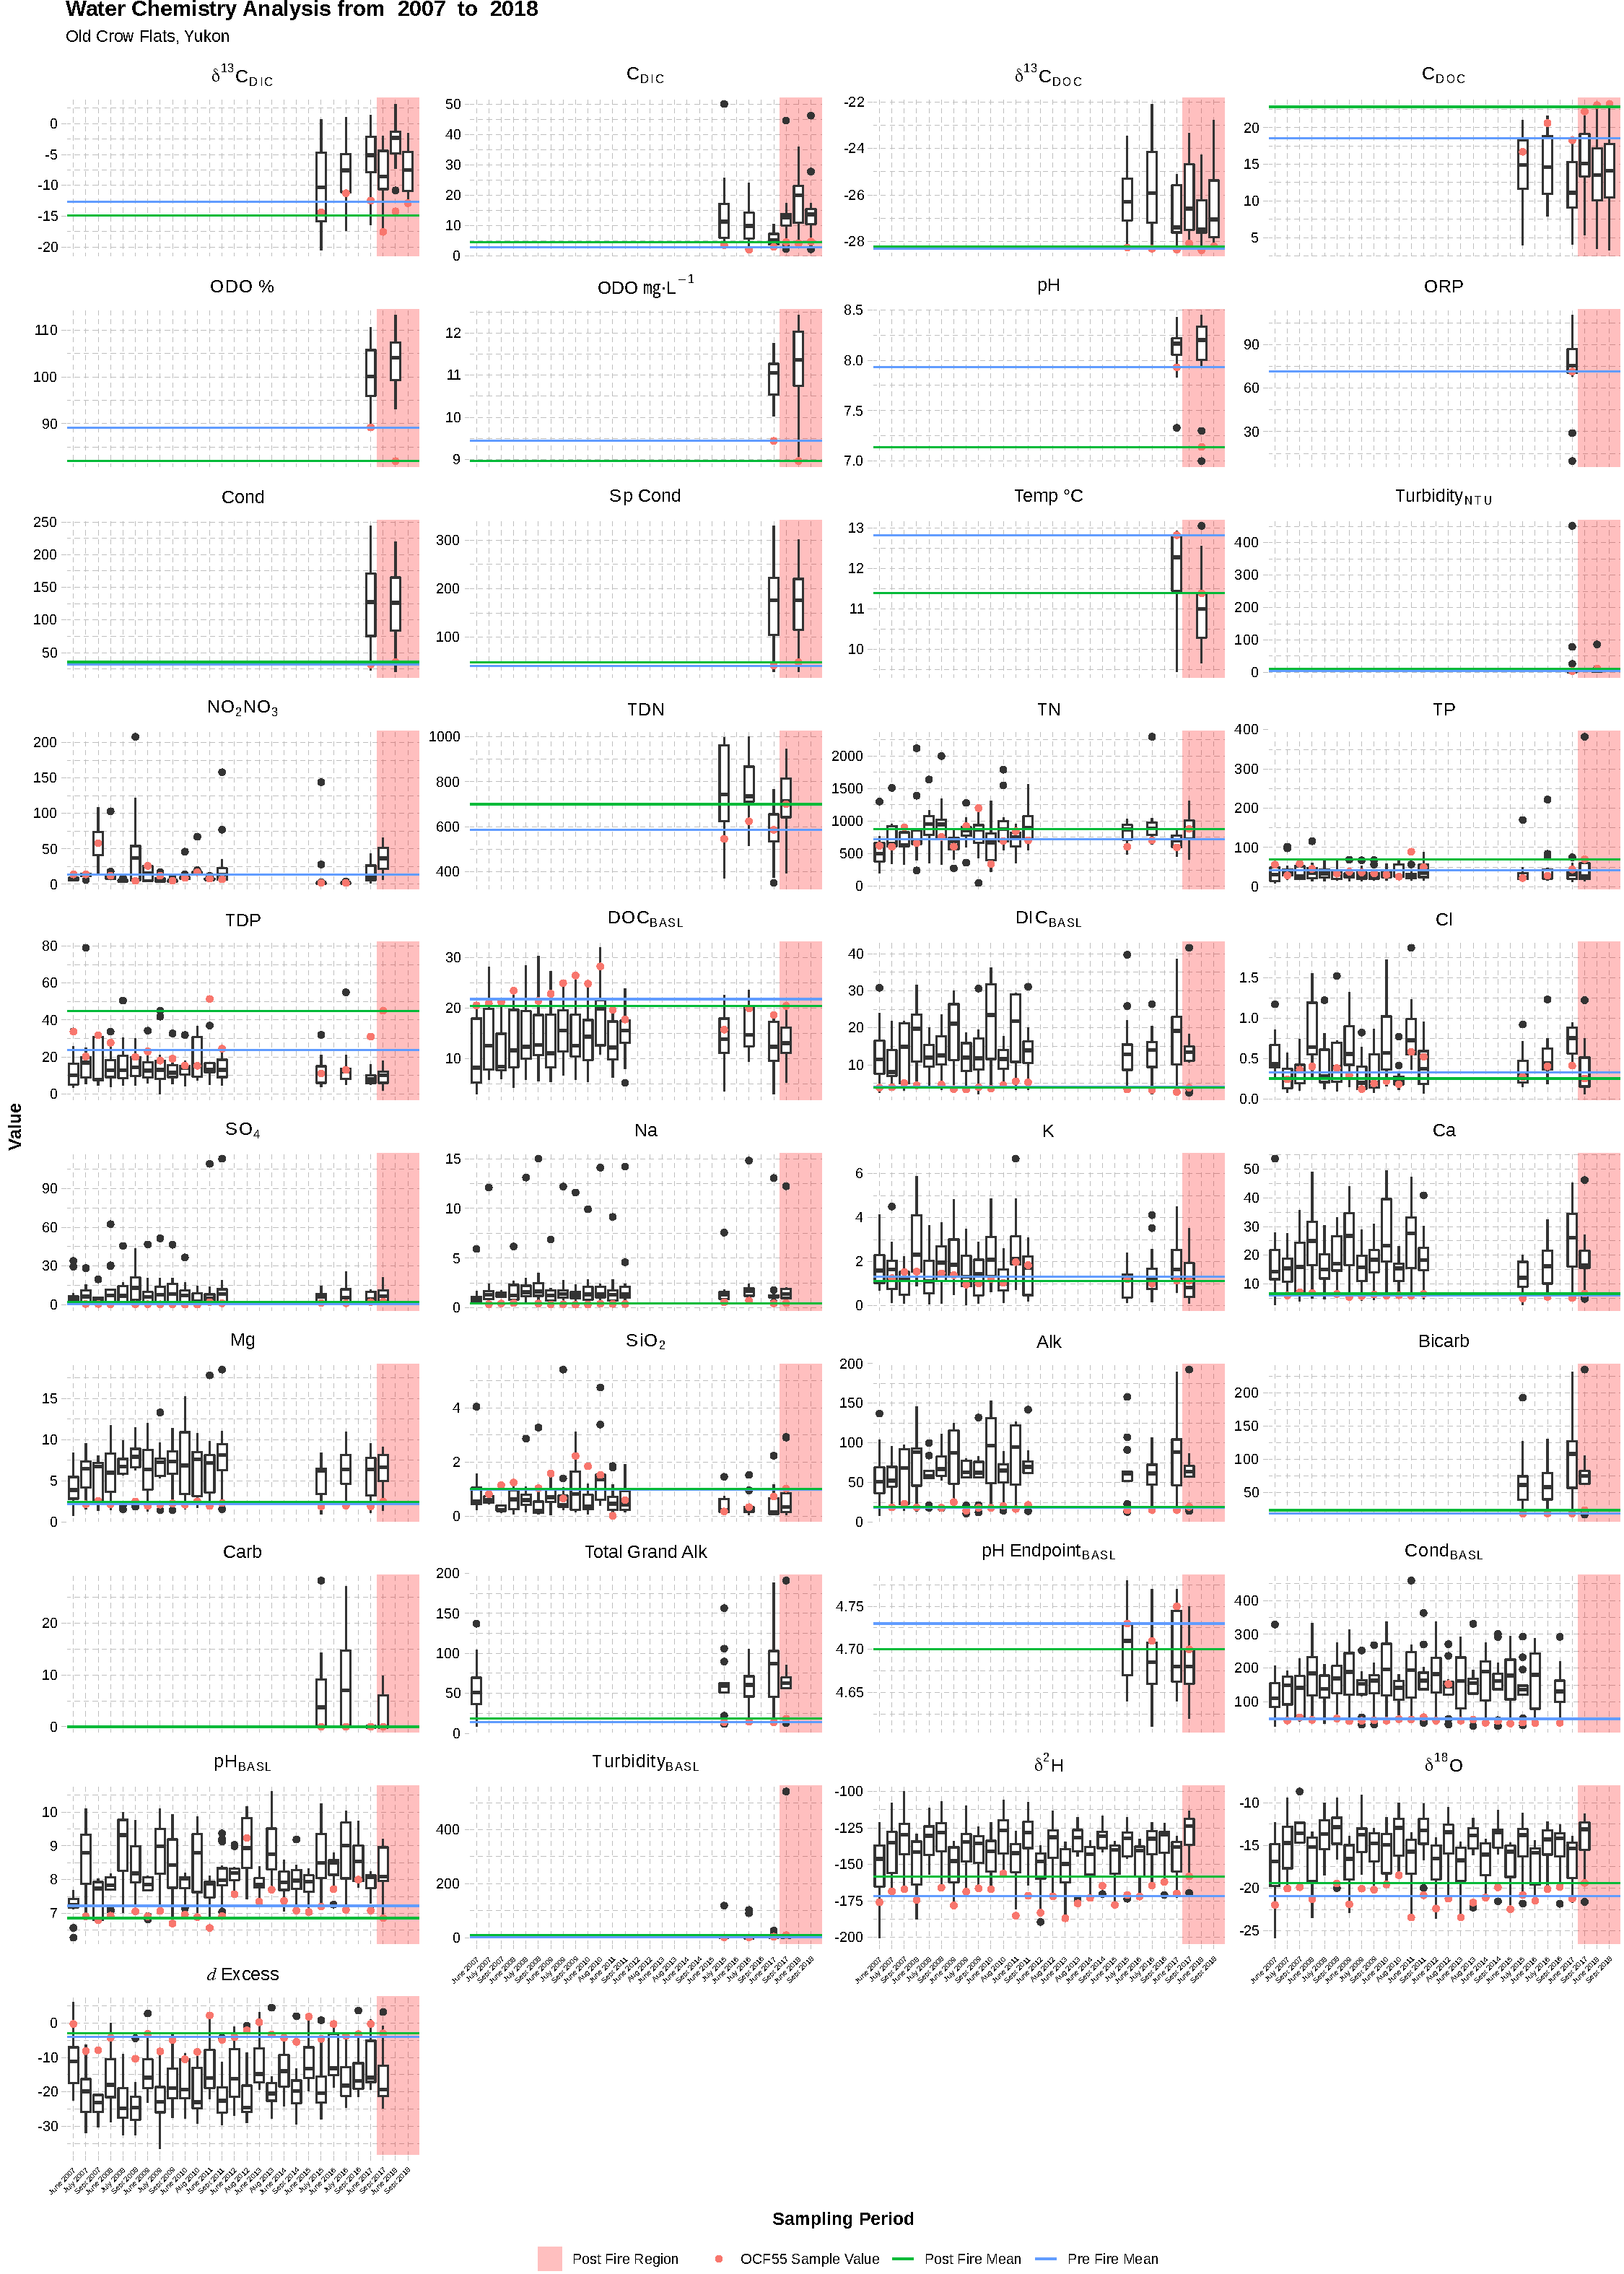
\includegraphics[width=0.8\linewidth]{Figures/figure2} 

}

\caption{This is a messy graphic right now but I will clean it up in the future.}\label{fig:unnamed-chunk-4}
\end{figure}

Pellentesque habitant morbi tristique senectus et netus. Magnis dis
parturient montes nascetur ridiculus mus mauris vitae ultricies. Nibh
nisl condimentum id venenatis. Lorem ipsum dolor sit amet consectetur
adipiscing elit duis. Eget aliquet nibh praesent tristique magna sit
amet purus. Orci phasellus egestas tellus rutrum. Mauris cursus mattis
molestie a. Amet cursus sit amet dictum sit. Tellus id interdum velit
laoreet. Tortor at risus viverra adipiscing. Ullamcorper malesuada proin
libero nunc. Elit ullamcorper dignissim cras tincidunt lobortis feugiat
vivamus. Eget dolor morbi non arcu risus quis. Pulvinar pellentesque
habitant morbi tristique senectus.

\begin{figure}

{\centering 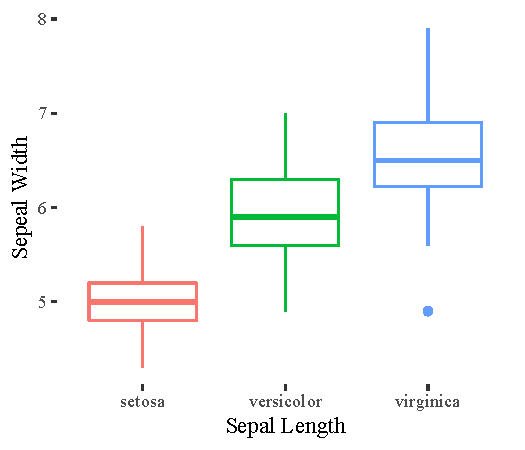
\includegraphics[width=0.65\linewidth]{skeleton_files/figure-latex/unnamed-chunk-5-1} 

}

\caption{Another figure showing how base R plots might look on this poster!}\label{fig:unnamed-chunk-5}
\end{figure}

More text now here Pellentesque habitant morbi tristique senectus et
netus. Magnis dis parturient montes nascetur ridiculus mus mauris vitae
ultricies. Nibh nisl condimentum id venenatis. Lorem ipsum dolor sit
amet consectetur adipiscing elit duis. Eget aliquet nibh praesent
tristique magna sit amet purus. Orci phasellus egestas tellus rutrum.
Mauris cursus mattis molestie a. Amet cursus sit amet dictum sit. Tellus
id interdum velit laoreet. Tortor at risus viverra adipiscing.
Ullamcorper malesuada proin libero nunc. Elit ullamcorper dignissim cras
tincidunt lobortis feugiat vivamus. Eget dolor morbi non arcu risus
quis. Pulvinar pellentesque habitant morbi tristique senectus.

\section{Next Steps}\label{next-steps}

Pellentesque habitant morbi tristique senectus et netus. Magnis dis
parturient montes nascetur ridiculus mus mauris vitae ultricies. Nibh
nisl condimentum id venenatis. Lorem ipsum dolor sit amet consectetur
adipiscing elit duis. Eget aliquet nibh praesent tristique magna sit
amet purus. Orci phasellus egestas tellus rutrum. Mauris cursus mattis
molestie a. Amet cursus sit amet dictum sit. Tellus id interdum velit
laoreet. Tortor at risus viverra adipiscing. Ullamcorper malesuada proin
libero nunc. Elit ullamcorper dignissim cras tincidunt lobortis feugiat
vivamus. Eget dolor morbi non arcu risus quis. Pulvinar pellentesque
habitant morbi tristique senectus.
\printbibliography
}
\end{multicols*}

%end the poster
\end{document}
